Durch das Vorgehen nach Abbildung \ref{tikz:abbKodierungUndDekodierung} und die beschriebenen Kodiermöglichkeiten kann die Zuordnung der Kamerapunkte und der Bildschirmpunkte erfolgen.
Mithilfe weiterer Schritte kann man daraus die Oberfläche rekonstruieren.
%
\begin{figure}[H]
	\centering
	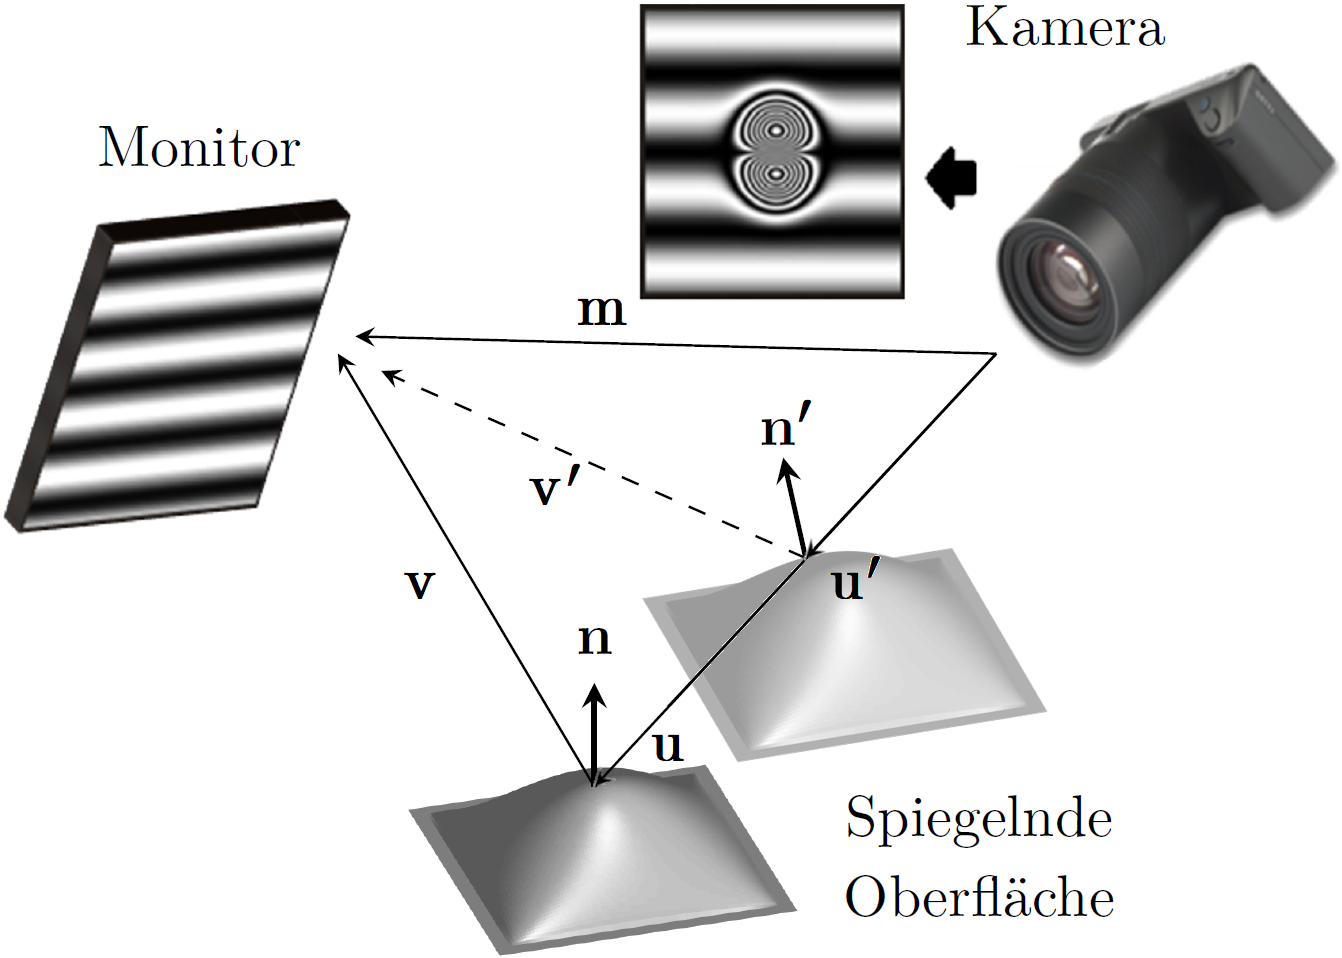
\includegraphics[width=0.7\textwidth]{02_grundlagenZurDeflektometrie/rekonstruktion/rekonstruktionUndRegularisierungsproblem/figures/regularisierungsproblem}
	\caption[Regularisierungsproblem]{Regularisierungsproblem. \textit{in Anlehnung an} \cite{stereoDeflektometrie}}
	\label{img:regularisierungsproblem}
\end{figure}
%
\noindent
Abbildung \ref{img:regularisierungsproblem} zeigt die Strahlenverfolgung zur Bestimmung der Oberflächennormalen $n$.
Zunächst benötigt man neben der Zuordnung zusätzliche Informationen über den Systemaufbau.
Das umfasst die Positionen und Ausrichtungen der Kamera und des Monitors im Raum.
Dadurch ist der Vektor $m$, sowie die Richtung des Sichtvektors $u$ bestimmt.
Man weiß zwar welcher Kamerapunkt welchen Punkt des Bildschirms sieht, allerdings ist dadurch das optische System nicht ausreichend beschrieben um die Länge des Sichtvektors $u$ anzugeben.
Es fehlt die Lage der Oberfläche.
Wäre diese bekannt, könnte der Reflexionsvektor $v$ mit 
\begin{equation*}
	v = m - u
\end{equation*}
bestimmt werden.
Mithilfe des Reflexionsgesetzes kann man aus dem Reflexionsvektor $v$ und dem Sichtvektor $u$ den Normalenvektor $n$ bestimmen:
%
\begin{equation}
	n = \dfrac{v - u}{\left\Vert v - u \right\Vert}	
\end{equation}
%
Durch die Unbestimmtheit des Sichtvektors $u$, erhält man entlang seiner Richtung unendlich viele potentielle Normalenvektoren $n$ des beobachteten Oberflächenpunkts.
Das heißt, es gibt unendlich viele mögliche Positionen des Oberflächenpunkts entlang der Sichtrichtung.
Diese Mehrdeutigkeit wird als Regularisierungs- oder Deflektometrieproblem bezeichnet \cite{regularisierungsproblem}.

%TODO Regularisierungsverfahren beschreiben? z. B. Stereo-Verfahren
\p
Schließlich ist es möglich, aus diesem Normalenfeld die räumlichen Informationen der Oberfläche zu berechnen.
Dafür kann man zunächst aus den Normalenvektoren die zugehörigen Tangentialebenen berechnen, die über je zwei Richtungsvektoren definiert sind.
Diese Richtungsvektoren bilden die Tangentialfelder des Prüfobjekts.
Man kann über eine Integration der Tangentialfelder in ausgewählte Richtungen Kurven bestimmen, die in der Oberfläche des Objekts liegen.
Durch diese Integration erhält man einen Höhenzusammen\-hang der Oberflächenpunkte.
Wenn zusätzlich ein Oberflächenpunkt gegeben ist, kann man die dreidimensionalen Positionen der Oberflächenpunkte im Raum angeben \cite{kit_werling}.